\subsubsection{Results}

At the end, we need to evaluate the model in order to get the results. We pass in our model, test data and location where we want results to be saved. The function (that is split into parts 1-4) then evaluates the model and results are available to us.
\begin{listing}[H]
\caption{Evaluate model model function -part 1}
\begin{minted}{python}
def evaluate_model(model, x_test, y_test, file_Path):
    test_data = spark.createDataFrame
                (pd.concat([x_test, y_test], axis=1))

    platform_indexer = StringIndexer(inputCol="platformType", 
                                    outputCol="platformIndex")
    test_data = platform_indexer.fit(test_data).transform(test_data)

    assembler = VectorAssembler(inputCols=["platformIndex"], 
                                outputCol="features")
    test_data = assembler.transform(test_data)

    predictions = model.transform(test_data)

    evaluator = MulticlassClassificationEvaluator(labelCol="label", 
                                        predictionCol="prediction")

    class_labels = test_data.select("label").distinct()
                    .rdd.flatMap(lambda x: x).collect()
    metrics = {}

\end{minted}
\end{listing}

\begin{listing}[H]
\caption{Evaluate model model function -part 2}
\begin{minted}{python}
    for label in class_labels:
        evaluator.setMetricName("accuracy")
        evaluator.setMetricLabel(label)
        accuracy = evaluator.evaluate(predictions)

        evaluator.setMetricName("weightedPrecision")
        evaluator.setMetricLabel(label)
        precision = evaluator.evaluate(predictions)

        evaluator.setMetricName("weightedRecall")
        evaluator.setMetricLabel(label)
        recall = evaluator.evaluate(predictions)

        evaluator.setMetricName("weightedFMeasure")
        evaluator.setMetricLabel(label)
        f1_score = evaluator.evaluate(predictions)

\end{minted}
\end{listing}

\begin{listing}[H]
\caption{Evaluate model model function -part 3}
\begin{minted}{python}
        metrics[label] = {"accuracy": accuracy, "precision": precision, 
                          "recall": recall, "f1-score": f1_score}

    predictionAndLabels = predictions.select("prediction", "label").rdd
    multiclass_metrics = MulticlassMetrics(predictionAndLabels)
    confusion_matrix = multiclass_metrics.confusionMatrix().toArray()

    label_counts = predictionAndLabels.map(lambda x: (x[1], 1))
                   .reduceByKey(lambda x, y: x + y).collectAsMap()
    support = {label: label_counts.get(label, 0) for label in class_labels}

    metrics_table = pd.DataFrame.from_dict(metrics, orient="index")
    print("Metrics per Class:")
    print(metrics_table)

    support_table = pd.DataFrame.from_dict
                    (support, orient="index", columns=["Support"])
    print("Support:")
    print(support_table)

    fig, ax = plt.subplots()
    im = ax.imshow(confusion_matrix, cmap="Blues")

    tick_labels = np.arange(len(class_labels))
    ax.set_xticks(tick_labels)
    ax.set_yticks(tick_labels)
    ax.set_xticklabels(class_labels, rotation=45)
    ax.set_yticklabels(class_labels)
    plt.xlabel("Predicted")
    plt.ylabel("Actual")
\end{minted}
\end{listing}

\begin{listing}[H]
\caption{Evaluate model model function -part 4}
\begin{minted}{python}
    cbar = ax.figure.colorbar(im, ax=ax)
    cbar.ax.set_ylabel("Count", rotation=-90, va="bottom")

    for i in range(len(class_labels)):
        for j in range(len(class_labels)):
            text = ax.text(j, i, int(confusion_matrix[i, j]), 
                           ha="center", va="center", color="w")

    plt.title("Confusion Matrix")
    
    metrics_table.to_csv(file_Path + "/metrics.csv")
    plt.savefig(file_Path + "/confusion_matrix.png")

    plt.close()
\end{minted}
\end{listing}

\begin{figure}[H]
    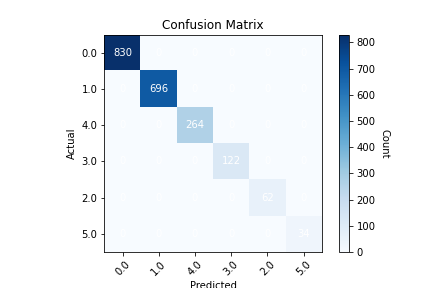
\includegraphics[scale=0.85]{img/Model/Classification/Dtree/confusion_matrix.png}
    \centering
    \caption{Decision tree confusion matrix}
    \label{fig:dtree_confusion_matrix}
\end{figure}